%%%%%%%%%%%%%%%%%%%%%%%%%%%%%%%%%%%%%%%%%%%%%%%%%%%%%%%%%%%%%%%%%%%%%%%%%%%%%%%%%%%%%%%%%%%%%%%%%%%%%%%%%%%%%%%%%%%%%%%%%%%%%%%%%%%%%%%%%%%%%%%%%%%%%%%%%%%
% This is just an example/guide for you to refer to when submitting manuscripts to Frontiers, it is not mandatory to use frontiers.cls nor frontiers.tex  %
% This will only generate the Manuscript, the final article will be typeset by Frontier after acceptance.                                                 %
%%%%%%%%%%%%%%%%%%%%%%%%%%%%%%%%%%%%%%%%%%%%%%%%%%%%%%%%%%%%%%%%%%%%%%%%%%%%%%%%%%%%%%%%%%%%%%%%%%%%%%%%%%%%%%%%%%%%%%%%%%%%%%%%%%%%%%%%%%%%%%%%%%%%%%%%%%%

%%% Version 2.0 Generated 2013/09/12 %%%
%%% You will need to have the following packages installed: datetime, fmtcount, etoolbox, fcprefix, which are normally inlcuded in WinEdt. %%%
%%% In http://www.ctan.org/ you can find the packages and how to install them, if necessary. %%%

%\documentclass{frontiersENG} % for Engineering articles
\documentclass{frontiersSCNS} % for Science articles
%\documentclass{frontiersMED} % for Medicine articles

\usepackage{url,lineno}
\usepackage{graphicx}
\usepackage{minted}
\linenumbers


% Leave a blank line between paragraphs in stead of using \\

\copyrightyear{2013}
\pubyear{2013}

\def\journal{Neuroinformatics}%%% write here for which journal %%%
\def\DOI{}
\def\articleType{Methods}
\def\keyFont{\fontsize{8}{11}\helveticabold }
\def\firstAuthorLast{Nunez-Iglesias {et~al.}} %use et al only if is more than 1 author
\def\Authors{Juan Nunez-Iglesias\,$^{1,2,*}$, Ryan Kennedy\,$^{1,3}$, Stephen M. Plaza\,$^{1}$, Anirban Chakraborty\,$^{4}$ and William T. Katz\,$^1$}
% Affiliations should be keyed to the author's name with superscript numbers and be listed as follows: Laboratory, Institute, Department, Organization, City, State abbreviation (USA, Canada, Australia), and Country (without detailed address information such as city zip codes or street names).
% If one of the authors has a change of address, list the new address below the correspondence details using a superscript symbol and use the same symbol to indicate the author in the author list.
\def\Address{$^{1}$FlyEM project, HHMI Janelia Farm Research Campus, Ashburn, VA, USA \\
$^{2}$ Present address: Life Sciences Computation Centre, Victorian Life Sciences Computation Initiative, Carlton, VIC, Australia \\
$^{3}$ Department of Computer and Information Science, School of Engineering and Applied Sciences, University of Pennsylvania, Philadelphia, PA, USA \\
$^{4}$ Video Computing Group, Department of Electrical Engineering, University of California at Riverside, Riverside, CA, USA}
% The Corresponding Author should be marked with an asterisk
% Provide the exact contact address (this time including street name and city zip code) and email of the corresponding author
\def\corrAuthor{Juan Nunez-Iglesias}
\def\corrAddress{Life Sciences Computation Centre, Victorian Life Sciences Computation Initiative, Carlton, VIC, Australia}
\def\corrEmail{juan.n@unimelb.edu.au}

% \color{FrontiersColor} Is the color used in the Journal name, in the title, and the names of the sections.


\begin{document}
\onecolumn
\firstpage{1}

\title[learned agglomeration]{Graph-based Active Learning of Agglomeration (GALA): a Python library to segment 2D and 3D neuroimages.}
\author[\firstAuthorLast]{\Authors}
\address{}
\correspondance{}
\extraAuth{}% If there are more than 1 corresponding author, comment this line and uncomment the next one.
%\extraAuth{corresponding Author2 \\ Laboratory X2, Institute X2, Department X2, Organization X2, Street X2, City X2 , State XX2 (only USA, Canada and Australia), Zip Code2, X2 Country X2, email2@uni2.edu}
\topic{Python in Neuroscience II}% If your article is part of a Research Topic, please indicate here which.

\maketitle

%%%%%%%%%%%%%%%%%%%%%%%%%%%%%%%%%%%%%%%%%%%%%%%%%%%%%%%%%%%%%%%%%%%%%%%%%%%%%%%%%%%%%%%%%%%%%%%%%%%%%%%%%%%%%%%%%%%%%%%%%%%%%%%%%%%%%%%%%%%%%%%%%%%%%%%%%%%%%%%%%%%%%%%%%%%%%%%%%%%%%%%%%%%%%%%%%%%%%%%%%%%%%%%%%%%%%%%%%%%%%%%%%%%%%%%
%%% The sections below are for reference only.
%%%
%%% For Original Research Articles, Clinical Trial Articles, and Technology Reports the following sections are mandatory:
%%% Abstract, Introduction, Material and Methods, Results, and Discussion.
%%% Please note that the Material and Methods section can be placed in any of the following ways: before Results, before Discussion or after Discussion.
%%%
%%% For Clinical Case Studies the following sections are mandatory: Abstract, Introduction, Background, Discussion, and Concluding Remarks.
%%%
%%% For all other article types there are no mandatory sections.
%%%%%%%%%%%%%%%%%%%%%%%%%%%%%%%%%%%%%%%%%%%%%%%%%%%%%%%%%%%%%%%%%%%%%%%%%%%%%%%%%%%%%%%%%%%%%%%%%%%%%%%%%%%%%%%%%%%%%%%%%%%%%%%%%%%%%%%%%%%%%%%%%%%%%%%%%%%%%%%%%%%%%%%%%%%%%%%%%%%%%%%%%%%%%%%%%%%%%%%%%%%%%%%%%%%%%%%%%%%%%%%%%%%%%%%

\begin{abstract}

The aim in high-resolution connectomics is to reconstruct complete neuronal connectivity in a tissue.
Currently, the only technology capable of resolving the smallest neuronal processes is electron microscopy (EM).
Thus, a common approach is to perform (error-prone) automatic segmentation of EM images, followed by manual proofreading by experts to fix errors.
We have developed an algorithm and software library to not only improve the accuracy of the initial automatic segmentation, but also point out the image coordinates where it is likely to have made errors.
Our software, called gala (graph-based active learning of agglomeration), improves the state of the art in agglomerative image segmentation.
It is implemented in Python and makes extensive use of the scientific Python stack (numpy, scipy, networkx, scikit-learn, scikit-image, and others).
We present here the software architecture of the gala library, and discuss several designs that we consider would be generally useful for other segmentation packages.
We also discuss the current limitations of the gala library and how we intend to address them.

%%% Leave the Abstract empty if your article falls under any of the following categories: Editorial Book Review, Commentary, Field Grand Challenge, Opinion or specialty Grand Challenge.
\section{}
%As a primary goal, the abstract should render the general significance and conceptual advance of the work clearly accessible to a broad readership. References should not be cited in the abstract.


\tiny
 \keyFont{ \section{Keywords:} connectomics, python, electron microscopy, image segmentation, machine learning} %All article types: you may provide up to 8 keywords; at least 5 are mandatory.
\end{abstract}


\section{Introduction}

% For Original Research Articles, Clinical Trial Articles, and Technology Reports the introduction should be succinct, with no subheadings.
%
%For Clinical Case Studies the Introduction should include symptoms at presentation, physical exams and lab results.
%

Connectomics, the elucidation of complete neuronal circuits, requires resolutions as low as 5-10nm to distinguish the smallest neuronal processes, but also fields of view hundreds of micrometers across or more, as neurons can easily span those distances.
This size disparity results in large image volumes of at least 10 gigavoxels and often orders of magnitude larger.
Neurons can then be thought of as segments in this image.
Combining an accurate segmentation with the position of pre- and post-synaptic sites in the image \citep{Kreshuk:2011el, Jagadeesh:2013wn}, one can obtain the shapes, locations, and connectivity of all the neurons in an image volume.

Until recently, the rate-limiting step has been the proofreading of the automatic segmentation  \citep{Chklovskii:2010df}.
In response, we developed a new machine learning-based algorithm for image segmentation \citep{NunezIglesias:2013cd} which, in addition to providing state of the art automatic segmentation accuracy, directs proofreaders to likely areas of error in the segmentation.
This has dramatically sped up proofreading and reconstruction speed (5-16-fold, in our anecdotal observations).

The algorithm, called GALA (graph-based active learning of agglomeration), works by repeatedly consulting a gold standard segmentation (prepared by human annotators) as it agglomerates sub-segments according to its current best guess.
(Note: throughout this paper, we will use "GALA" to describe the algorithm, and "gala" or "Gala" for the Python library and software.)
It therefore accumulates a training dataset that prevents it from repeating past mistakes.
Furthermore, through the probability output of the classifier, it can estimate its own confidence in whether two segments should be merged, and this estimate can be used for proofreading.

GALA outperformed previous agglomeration methods in EM and natural image segmentation \citep{NunezIglesias:2013cd}, and it remains top-ranked in the SNEMI3D challenge, over tools developed specifically for anisotropic data \citep{snemi, Liu:2012ba, Kaynig:2013tv}.
See Figure \ref{fig:01} for two segmentation examples obtained with the gala library.

In this paper, we briefly present the Python application programming interface (API) and the command-line interface (CLI), before delving more deeply into particularly useful design choices, and finally discussing the current limitations of the library and future directions.


\begin{figure}
\begin{center}
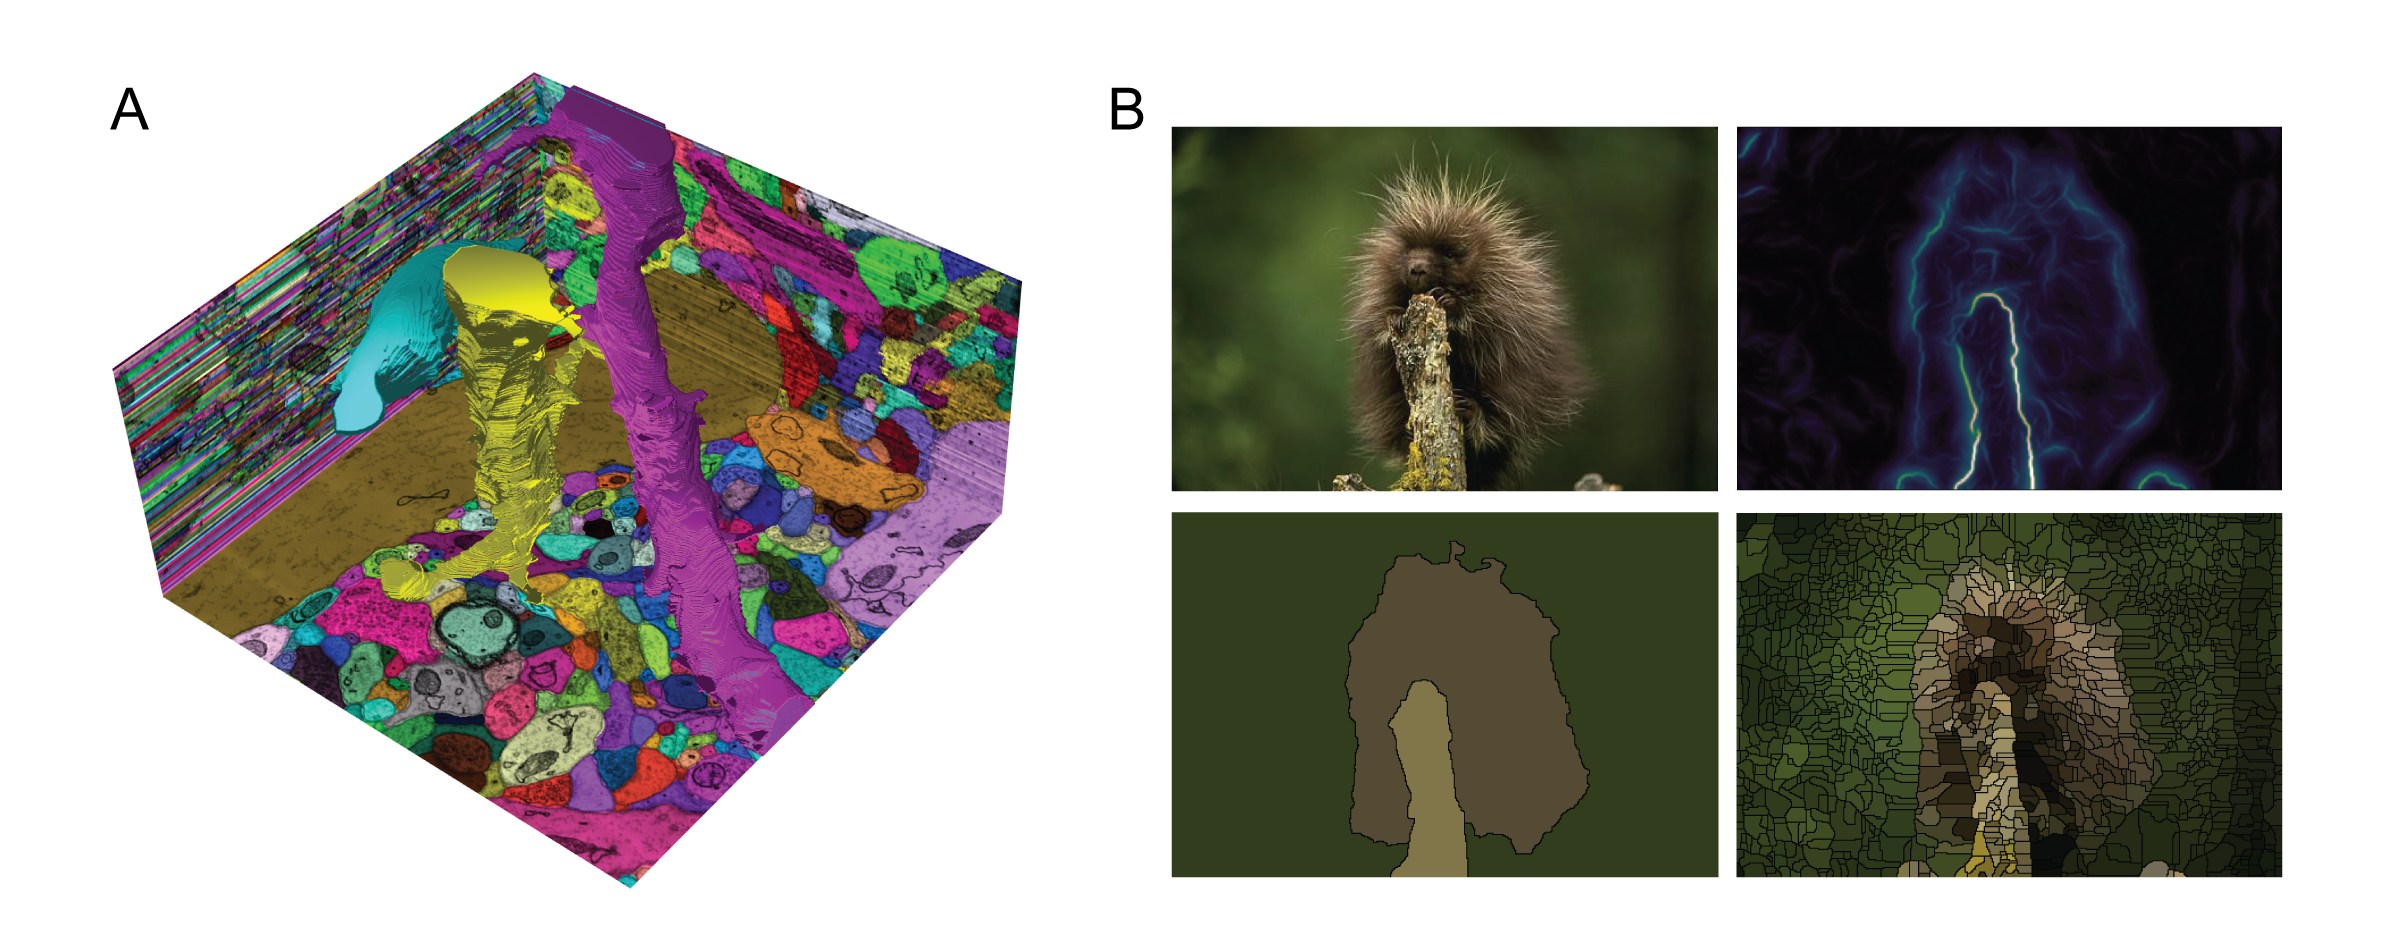
\includegraphics[width=18cm]{figure1}
\end{center}
 \textbf{\refstepcounter{figure}\label{fig:01} Figure \arabic{figure}.}{ Two sample automatic segmentations performed with gala. (A) The SNEMI3D test data. (B) Our favorite fuzzball from the Berkeley Segmentation Data Set. }
\end{figure}


\section{API}


\subsection{Python API}

GALA has three main prerequisites:
\begin{itemize}
\item a pixel-level \emph{probability map}, usually the \emph{probability of boundary}; and
\item a \emph{superpixel map} (or supervoxel), an initial fine-grained segmentation; and
\item a \emph{gold standard segmentation}, that represents the true segmentation of a training volume.
\end{itemize}

For the first requirement, we have used Ilastik \citep{ilastik} in our own work on EM images, gPb \citep{globalpb} for natural images, or the probability maps provided by \cite{Ciresan:2012vi} for the SNEMI3D challenge.
As you can see, gala is agnostic about the origin of the input probability maps, both theoretically and in this implementation.
Furthermore, these can have any number of channels, such as probability of various other kinds of pixel types (mitochondria, vesicles, glia) or the output of texture filters at that pixel.

For the second point, we have used the watershed algorithm \citep{Vincent:1991}, but other methods, such as SLIC \citep{Achanta:2012wc} would work.
Gala itself contains an implementation of watershed, although for some parameter sets we just wrap the implementation in \texttt{\small scikit-image}, which is more efficient and works both in 2D and 3D.
Again, the only requirement here is that the input volume is partitioned into some integer labeled regions.
The algorithm that generated the partition is not important.

The final requirement is a completely segmented image to be used as ground truth.
For neuronal EM images, we used ground truth segmentation generated with the open-source Raveler software \citep{raveler}, while a large ground truth body exists with the Berkeley Segmentation Data Set (BSDS) \citep{MartinFTM01}.
For other images, such as 3D fluorescence microscopy images, generation of ground truth can be a laborious process.
This has indeed become the rate-limiting step in a gala segmentation, so we are moving to eliminate this requirement so that only a subset of ground truth is needed (see discussion).

Given the above, we create a region adjacency graph, or RAG (implemented in \texttt{\small gala.agglo.Rag}) corresponding to the training superpixel and probability maps, and perform repeated training agglomerations of the superpixels while comparing against the ground truth (\texttt{\small Rag.learn\_agglomerate}).
This produces a training set, to which we can fit a classifier, which will then prioritize merges in a test volume to segment.
These operations are illustrated in the following code snippet, which can be run from gala's \texttt{\small tests/example-data} directory:

{\small
\begin{minted}[samepage=true]{python}
# imports
from gala import imio, classify, features, agglo, evaluate as ev
# read in training data
gt_train, pr_train, ws_train = (map(imio.read_h5_stack,
                                ['train-gt.lzf.h5', 'train-p1.lzf.h5',
                                 'train-ws.lzf.h5']))
# create a feature manager
fm = features.moments.Manager()
fh = features.histogram.Manager()
fc = features.base.Composite(children=[fm, fh])
# create graph and obtain a training dataset
g_train = agglo.Rag(ws_train, pr_train, feature_manager=fc)
(X, y, w, merges) = g_train.learn_agglomerate(gt_train, fc)[0]
y = y[:, 0] # gala has 3 truth labeling schemes, pick the first one
# train a classifier, scikit-learn syntax
rf = classify.DefaultRandomForest().fit(X, y)
# a policy is the composition of a feature map and a classifier
learned_policy = agglo.classifier_probability(fc, rf)
# get the test data and make a RAG with the trained policy
pr_test, ws_test = (map(imio.read_h5_stack,
                        ['test-p1.lzf.h5', 'test-ws.lzf.h5']))
g_test = agglo.Rag(ws_test, pr_test, learned_policy, feature_manager=fc)
g_test.agglomerate(0.5) # best expected segmentation
seg_test1 = g_test.get_segmentation()
\end{minted}
}

We've made gala \emph{multichannel agnostic}, so that \texttt{\small agglo.Rag} and all of the existing feature managers can receive as input a multichannel probability map and transparently compute the corresponding features.

{\small
\begin{minted}[samepage=true]{python}
# the same approach works with a multi-channel probability map
p4_train = imio.read_h5_stack('train-p4.lzf.h5')
# note: the feature manager works transparently with multiple channels!
g_train4 = agglo.Rag(ws_train, p4_train, feature_manager=fc)
(X4, y4, w4, merges4) = g_train4.learn_agglomerate(gt_train, fc)[0]
y4 = y4[:, 0]
rf4 = classify.DefaultRandomForest().fit(X4, y4)
learned_policy4 = agglo.classifier_probability(fc, rf4)
p4_test = imio.read_h5_stack('test-p4.lzf.h5')
g_test4 = agglo.Rag(ws_test, p4_test, learned_policy4, feature_manager=fc)
g_test4.agglomerate(0.5)
seg_test4 = g_test4.get_segmentation()
\end{minted}
}

Because gala was created as research software, it implements a number of additional agglomerative segmentation algorithms, including mean boundary, oriented mean boundary \citep{Arbelaez:jg}, median boundary, superpixel affinity learning \citep{Ren:2003jg} (which we also call "flat" learning), and LASH \citep{Jain:2011vr}.

{\small
\begin{minted}[samepage=true]{python}
g_testm = agglo.Rag(ws_test, pr_test,
                    merge_priority_function=agglo.boundary_mean)
g_testm.agglomerate(0.5)
seg_testm = g_testm.get_segmentation()
\end{minted}
}

\subsection{Segmentation evaluation module}

One of the most generally reusable parts of the gala library is the evaluation module in \texttt{\small gala/evaluate.py}.
It offers efficient implementations of edit distance, Rand Index \citep{Rand:1971uy}, Adjusted Rand Index \citep{Hubert:1985}, Fowlkes-Mallows index \citep{Fowlkes:1983wz}, and Variation of Information (VI) \citep{meila:2005}.
Among these, we focused the most effort on the VI metric for its numerous advantages \citep{meila:2005, NunezIglesias:2013cd}.
The two components of VI are computed quickly and efficiently with the \texttt{\small evaluate.split\_vi} function.

{\small
\begin{minted}[samepage=true]{python}
gt_test = imio.read_h5_stack('test-gt.lzf.h5')
import numpy as np
results = np.vstack((
    ev.split_vi(ws_test, gt_test),
    ev.split_vi(seg_testm, gt_test),
    ev.split_vi(seg_test1, gt_test),
    ev.split_vi(seg_test4, gt_test)
    ))
\end{minted}
}

This should have an output like:

{\small
\begin{minted}[samepage=true]{python}
print(results)
[[ 0.1845286   1.64774412]
 [ 0.18719817  1.16091003]
 [ 0.33793257  0.28697057]
 [ 0.33573312  0.23727755]]
 \end{minted}
}

Computing a set of VIs from an ultrametric contour map (UCM) \citep{Arbelaez:jg} is easily done with the \texttt{\small vi\_by\_threshold} function.
From this we can generate the split VI plot (figure \ref{fig:02}) that we introduced in \cite{NunezIglesias:2013cd}, showing the tradeoff between oversegmentation and undersegmentation.
This is in contrast to the commonly used plot of VI against segmentation threshold (see, e.g., \cite{Andres:2012vp}).


{\small
\begin{minted}[samepage=true]{python}
# generate split-vi plots for each method
from matplotlib import pyplot as plt
g_test.agglomerate(np.inf)
g_test4.agglomerate(np.inf)
g_testm.agglomerate(np.inf)
ucms = [g.get_ucm() for g in [g_testm, g_test, g_test4]]
vis = [ev.vi_by_threshold(u, gt_test, [0], [0])[1:] for u in ucms]
colors = ['black', 'deepskyblue', 'orange']
plt.figure(figsize=(3.3, 3.3))
from gala import viz
viz.plot_split_vi(vis, colors=colors)
plt.xlim(0, 1); plt.ylim(0, 1)
plt.legend(['mean agglomeration', 'gala 1-channel', 'gala 4-channel'],
           loc=1, fontsize=8)
plt.xticks(np.arange(0, 1.01, 0.2), fontsize=10)
plt.yticks(np.arange(0, 1.01, 0.2), fontsize=10)
plt.xlabel('false merges (bits)', fontsize=10)
plt.ylabel('false splits (bits)', fontsize=10)
plt.savefig('split-vi.png', dpi=300, bbox_inches='tight')
\end{minted}
}

\begin{figure}
\begin{center}
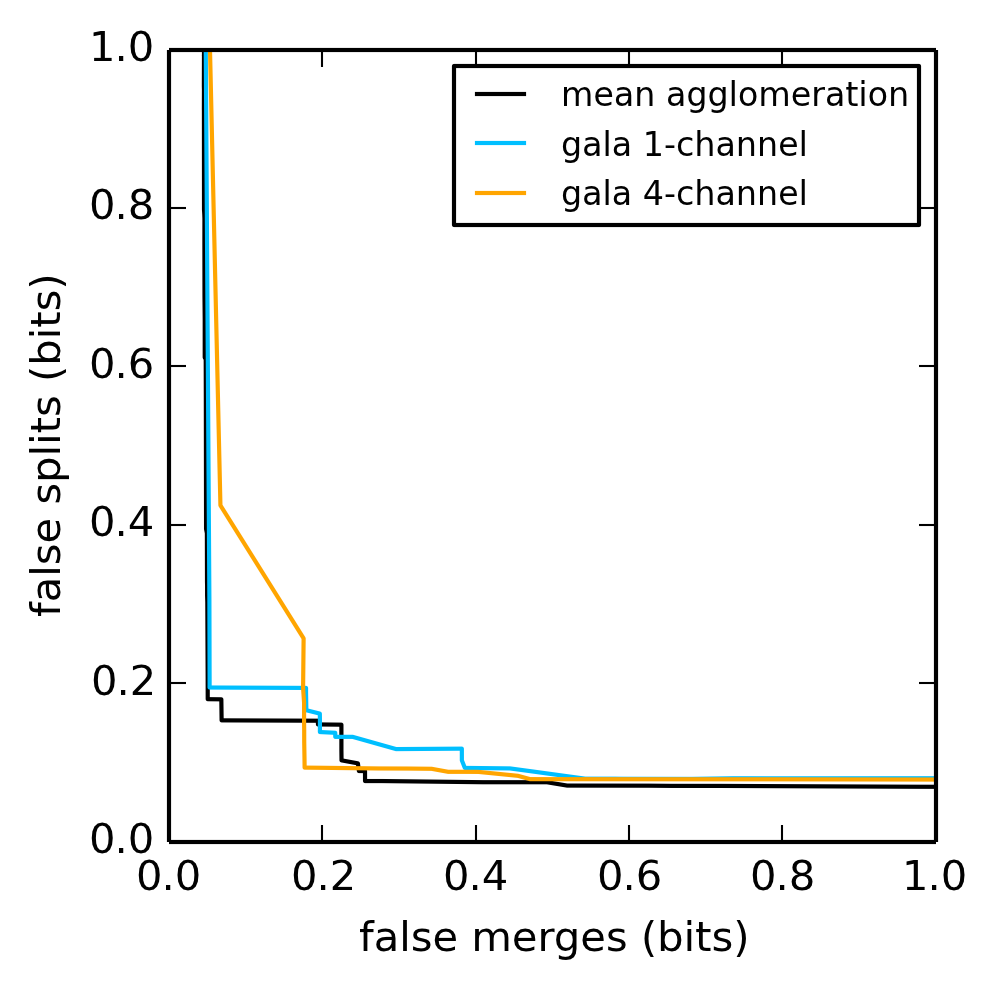
\includegraphics[width=85mm]{figure2}
\end{center}
 \textbf{\refstepcounter{figure}\label{fig:02} Figure \arabic{figure}.}{ The split VI plot for our sample data. Lower and to the left is better. One should \emph{not} conclude that mean agglomeration is the best technique, since this plot was generated with a tiny sample dataset. For a scientific comparison, see \cite{NunezIglesias:2013cd}. }
\end{figure}

\subsection{Command-line interface}

In addition to the flexible Python library interface, we developed a set of command-line scripts to perform common gala functions, such as training and segmenting.
This is the primary way of interacting with gala in a production environment.
For example, after determining suitable watershed parameters in an IPython environment \citep{Perez:2007}, these two commands produced our currently top-ranked entry to the SNEMI3D challenge \citep{snemi}:

{\small
\begin{minted}[samepage=true]{bash}
$ ~/projects/gala/bin/gala-train -e 5 \
    -F 'features.base.Composite(children=[\
                       features.moments.Manager(), \
                       features.histogram.Manager(25, 0, 1, [0.1, 0.5, 0.9]), \
                       features.graph.Manager()])' \
    -w train-2d-watershed.lzf.h5 \
    --output-dir ~/data/snemi3d/ \
    --experiment-name sn2d-opt \
    --no-channel-data \
    train-probabilities.lzf.h5 train-labels.lzf.h5 

$ ~/projects/gala/bin/gala-segment -C \
    -F 'features.base.Composite(children=[\
                       features.moments.Manager(), \
                       features.histogram.Manager(25, 0, 1, [0.1, 0.5, 0.9]), \
                       features.graph.Manager()])' \
    -w test-2d-watershed.lzf.h5 \
    --output-dir ~/data/snemi3d \
    -k sn2d-opt.classifier.h5 \
    -t `seq -s ' ' -f %.2f 0 0.01 1` \
    -R -J \
    --experiment-name sn2d-opt \
    test-probabilities.lzf.h5
\end{minted}
}

The commands, though onerous, are quite simple.
And, since they are based on \texttt{\small argparse}, both will provide helpful descriptions when presented with a \texttt{\small -h} flag.

In \texttt{\small gala-train}, \texttt{\small -e} indicates the number of training epochs (see \cite{NunezIglesias:2013cd} for details), \texttt{\small -F} indicates the feature manager, specified as a Python expression, and \texttt{\small -w} indicates the superpixel map.
The other options are self-explanatory, and finally, the two positional arguments are the probability map and the ground truth label volume.

\texttt{\small gala-segment} has similar options, with \texttt{\small -R} disabling the Raveler format \citep{raveler} used in Janelia and \texttt{\small -J} disabling NeuroProof JSON output (see section \ref{section:np} and \cite{np}).
Meanwhile, \texttt{\small -t} indicates the agglomeration thresholds at which segmentations should be output.

Finally, in addition to the command line interface, the options above are available through a JSON configuration file format.


\section{Design highlights}

The core of gala is the agglo.Rag class, which inherits from NetworkX's Graph class.
This region adjacency graph performs the agglomerative segmentation, whether learned or unsupervised.
However, its design is rather humdrum, so in this section we focus on a few design elements that we consider essential to gala's success.

\subsection{N-dimensional array support}

Many segmentation libraries assume 2D or 3D data, or provide separate functions for each (see, for example, \cite{slic-website}, or many OpenCV functions).

We instead abstracted away the notion of a neighboring pixel (or voxel) with a \texttt{\small get\_neighbor\_idxs} function that depends only on the pixel coordinates, the shape of the array, and the connectivity parameter, defined as the number of dimensions one can simultaneously step along to get to a neighbor.
All operations in our algorithm depend only on the definition of the local neighborhood. 
It was thus feasible to design all of gala to be dimension-agnostic.
This allowed us to produce segmentations of the Berkeley segmentation dataset \citep{MartinFTM01} and a 3D EM dataset from the same code base.

Numpy's \texttt{\small ndarray} object in particular has made reasoning about n-dimensional data extremely easy.
We present below the \texttt{\small get\_neighbor\_idxs} function to illustrate the advantages provided by the Python, numpy, and the ndarray object.

{\small
\begin{minted}[samepage=true]{python}
def get_neighbor_idxs(ar, idxs, connectivity=1):
    strides = array(ar.strides)/ar.itemsize
    if connectivity == 1: 
        steps = (strides, -strides)
    else:
        steps = []
        for i in range(1, connectivity+1):
            prod = array(list(it.product(*([[1, -1]] * i))))
            i_strides = array(list(it.combinations(strides, i))).T
            steps.append(prod.dot(i_strides).ravel())
    return idxs[:, newaxis] + concatenate(steps)
\end{minted}
}

We highlight the niceties of doing this in Python:
\begin{itemize}
\item the strides and itemsize elements of numpy arrays make it very easy to compute on linear indices and thus in n-dimensions transparently.
\item the itertools module of the Python standard library gives us combinations of moving forward or back along each dimension of the array.
\item numpy's array broadcasting rules allow concise, fast computation of neighboring indices simultaneously for a large number of input indices.
\end{itemize}

A great many algorithms in computer vision can be parameterized by neighboring voxels.
Thus, we encourage developers to write these in n-dimensional logic from the start to increase the range of applications of their software.
Having said that, we assumed isotropic data, which has been limiting in some cases.

\subsection{Feature managers and feature caches}

An example of a critical feature when determining the probability that two segments should be merged is the average pixel-level probability of boundary \citep{Ren:2003jg}.
As segments are merged, the shared surface between them and their common neighbors increases, thereby making the average a more reliable estimate of the true probability of a boundary.
Recomputing the mean from scratch, however, results in quadratic time complexity, because we are repeatedly iterating over the same pixels after each merge.
Therefore, a more efficient strategy is to cache a sum of the pixel probabilities and the count of pixels examined.
Then, when two boundaries are combined, their probability sums are added together, as are their counts, and the new average probability can be computed by dividing the new sum by the new count, in constant time.
This caching turns a quadratic operation into a linear one.

The above concept can be generalized to \emph{any} feature.
We found that, in many cases, caching intermediate computations dramatically improved the time complexity of feature computation.
For example, to compute the \emph{variance} of the pixel probabilities, we must cache the sum of the \emph{squared} pixel probabilities, along with simple sum and counts.
To compute a histogram, we cache the unnormalised histogram, and each bin is summed when two boundaries are combined.

We therefore devised a single class, which we call a feature manager, that is responsible for defining the cached values, and for computing the feature vector from the cached values.
This has enabled less obvious features, including, for example, many based on the convex hull of the segment.
The convex hull feature manager stores as a cache the convex hull of each node.
When two nodes are merged, the resulting convex hull can be computed faster by starting from the two initial hulls, rather than from the newly formed segment.
The manager then uses the hull to compute features such as segment convexity, by comparing the volume of the convex hull to the volume of the segment.

Developing a feature manager is easy: subclassing \texttt{\small features.base.Null}, dropping the \texttt{.py} file in the features folder, and optionally updating the \texttt{\small \_\_init\_\_.py} for easy import.
As an example, a recently added feature manager is the so-called ``inclusiveness''.
In 3D EM images, it is not biologically plausible that one segment would be enclosed within another.
Early on, we developed the idea of removing these inclusions by automatically merging the enclosed segment to the enveloping one, regardless of merge priority.
However, we later realised that this is only the extremum of a continuous set of features that we called "inclusiveness".
These include, for a pair of nodes $u$ and $v$, the size of the boundary between $u$ and $v$ divided by the total size of all boundaries around $u$, as well as the size divided by all the boundaries around $v$.

The GitHub pull request creating this manager can be found at:

\url{https://github.com/jni/ray/pulls?direction=desc&page=1&sort=created&state=closed}

\subsection{Classifier abstraction}

Given the vast heterogeneity of our initial feature space, we wished to use a random forest (RF) as our classifier of choice.
\texttt{\small scikit-learn}, the present gold-standard in machine learning Python libraries, did not contain a RF implementation when we started building gala.
We therefore decided to use Vigra, a C++ image analysis and machine learning library with Python bindings.
However, we recognized that a cross-compatible interface across libraries would allow rapid testing of various machine learning techniques.
We therefore built a wrapper around Vigra to match \texttt{\small scikit-learn}'s estimator interface, particularly the \texttt{\small fit()}, \texttt{\small predict()}, and \texttt{\small predict\_proba()} methods.

Because of this, it is trivial to use different classifiers for the learning and agglomeration steps of \texttt{\small gala}.
In particular, we have been able to use the recently vastly improved \texttt{\small RandomForestClassifier} from \texttt{\small scikit-learn} version 0.14 with no code changes.

In short, by using established interfaces, we were able to future-proof our software.
We recommend that anyone looking to build software in the Python ecosystem take a long look at related libraries to match interfaces as closely as possible.


\section{Discussion}


\subsection{Complete gold standard requirement}

As currently implemented, gala requires a fully segmented volume from which to learn.
In our experiments, this has become the major bottleneck when starting segmentations on new data.
Therefore, a priority in gala development going forward is the ability to mask volumes so that partial ground truth can be used.

\subsection{Memory and time inefficiency}

Gala's implementation, based on NetworkX, is slow and has a high memory footprint.
However, many improvements are within easy reach.

Firstly, we currently store feature caches and compute feature vectors as separate arrays.
This results in a huge time overhead for large graphs due to memory allocation, and also in memory usage because of the dictionaries required to store all the separate arrays.
However, because we are performing a hierarchical agglomeration, we know that the number of nodes and edges is bounded by twice the initial number.
Therefore, we can pre-allocate an initial array of shape \texttt{\small (2 * n\_nodes, cache\_size)} for the node feature caches, and similarly for the edges, and use an incremental indexing scheme to keep track of which node or edge in the hierarchy uses which row of the array.

Additionally, the graph currently stores indices to the voxels comprising each node and boundary, which is unnecessary.
Space and time can be saved by keeping only a single voxel and rebuilding nodes using a flood fill.

Finally, we chose the heavy \texttt{\small Graph} class of the NetworkX library for its flexibility and fast node addition and removal.
However, this is ultimately unnecessary: we can store the original supervoxel graph using a much more efficient structure, such as \texttt{\small scipy.sparse.csc\_graph}, and maintain a merge tree.
The graph at any level of the hierarchy can be rapidly constructed from this.

\subsection{Alternate backends}
\label{section:np}

As a workaround for gala's memory efficiency issues, we developed an alternative interface called NeuroProof \citep{np}, which can be used as the backend for the gala algorithm by calling the \texttt{\small Stack} class in \texttt{\small gala.stack\_np} instead of \texttt{\small agglo.Rag}.
NeuroProof implements region adjacency graphs in C++, with an optional translation layer to the Boost Graph Library \citep{bgl}.
Unlike generic graph libraries such as NetworkX, NeuroProof is optimized to handle the specific operations of traversing an image label volume, constructing an adjacency graph, and merging graph nodes together.
This specialization leads to time and memory savings over NetworkX over and above those offered by a C++ implementation.
NeuroProof serializes the graph using a JSON format that contains a list of edges (node pairs) and a few relevant attributes, such as node sizes and edge weights.
(The reference \texttt{\small agglo.Rag} implementation can also output to this format.)
Currently, NeuroProof exists as a completely separate, more efficient alternative interface within the gala library.
In the future, we intend to unify the two interface, and possibly more, by using a backend selection mechanism at runtime.

\section{Conclusions}

Like most academic software, gala is a mixture of new algorithms, some good design, and a variety of questionable decisions left over from a time of different priorities, but we hope that the existing and future functionality, the better parts of the software, and the lessons learned will be of value to the wider research community.
Don Knuth's famous maxim that ``premature optimization is the root of all evil'' \citep{knuth74opt} should not be taken too much to heart: in our case, this has led to time and memory performance issues that have been difficult to resolve.
Still, gala's success in segmenting not only the isotropic EM volume for which it was designed \citep{Glasner:2011uk, NunezIglesias:2013cd}, but also the BSDS natural image dataset and the SNEMI3D anisotropic EM dataset, suggests that it will be useful for some time to come.


%%% Use this if adding the figures directly in the mansucript, if so, please remember to also upload the files when submitting your article
%%% There is no need for adding the file termination, as long as you indicate where the file is saved. In the examples below the files (logo1.jpg and logo2.eps) are in the Frontiers LaTeX folder
%%% If using *.tif files convert them to .jpg or .png

% \textbf{Figure 1.}{ Enter the caption for your figure here.  Repeat as  necessary for each of your figures.}\label{fig:01}% If you don't add the figures in the LaTeX files, please upload them when submitting the article.
%
%%% Frontiers will add the figures at the end of the provisional pdf automatically %%%



\bibliographystyle{frontiersSCNS} % for Science and Engineering articles
%\bibliographystyle{frontiersinMED} % for Medicine articles
\bibliography{frontiers.bib}

\end{document}
